\documentclass[conference,letterpaper]{IEEEtran}
\usepackage[T1]{fontenc}
\usepackage[utf8]{inputenc}
\usepackage{cite}
\usepackage{amsmath,amssymb}
\usepackage{graphicx}
\usepackage{booktabs}
\usepackage{url}
\usepackage[hidelinks]{hyperref}
\newcommand{\review}[2]{\par\noindent\textit{[HUMAN REVIEW REQUIRED: #1] #2}\par}
\title{Measuring Directed Documentation Structure with Normalized Magnetic Spectra}
\author{\IEEEauthorblockN{Rocker D'Antonio\IEEEauthorrefmark{1}, Dimitrios Michael Manias\IEEEauthorrefmark{2}}
\IEEEauthorblockA{Mississippi State University, Mississippi State, MS 39762, USA\quad
\IEEEauthorrefmark{1}\href{mailto:rd1174@msstate.edu}{rd1174@msstate.edu}\quad
\IEEEauthorrefmark{2}\href{mailto:dmanias@cse.msstate.edu}{dmanias@cse.msstate.edu}\\
ORCID: \IEEEauthorrefmark{1}\href{https://orcid.org/0009-0001-8444-1772}{0009-0001-8444-1772}\quad
\IEEEauthorrefmark{2}\href{https://orcid.org/0000-0003-4390-3093}{0000-0003-4390-3093}}}
\hypersetup{pdftitle={Measuring Directed Documentation Structure with Normalized Magnetic Spectra},
pdfauthor={Rocker D'Antonio; Dimitrios Michael Manias},pdfsubject={W02 measurement paper; internal draft awaiting author review}}
\begin{document}
\maketitle
\begin{abstract}
Answering procedural questions can require information from several documentation
pages. Hyperlink direction shapes the routes available to readers and retrieval
agents seeking the semantic context needed to answer. This work evaluates
an established symmetric normalized magnetic Laplacian as a documentation
measurement profile, with explicit graph views, ordinary connectivity comparators
and numerical qualification, implemented in the reusable RetrievalArena
framework introduced in this work. Across fourteen corpus snapshots, component profiles
reveal structural differences whose interpretation depends on connected coverage,
charge and topology.
Controlled directed-cycle reversals preserve the weighted undirected graph,
degrees, reciprocity, connectivity partitions and trophic incoherence. They produce
numerically resolved changes in ten corpora (54 of 77 selected reversals),
with magnitudes and localization varying by corpus. A whole-corpus Docker refinement application changes the profiles and
supplies observed use of editor-added links, without establishing improved retrieval
or answer quality. The study establishes orientation sensitivity, blind spots and the coverage
and localization checks needed for interpretation.
\end{abstract}
\begin{IEEEkeywords}
technical documentation, directed graphs, magnetic Laplacian, spectral measurement,
information access
\end{IEEEkeywords}
\section{Introduction}
\label{sec:introduction}

Technical documentation supports software configuration, operation and
troubleshooting for human operators and agentic systems. Hyperlinks connect
material across pages, representing a documentation corpus as a directed graph
with pages as vertices and links as directed edges.

This work investigates normalized magnetic spectra as candidate measurements of
directed link structure. Its objective is to determine which changes in link
organization the profile distinguishes, under which graph conditions it is
informative, and how it describes a documentation refinement whose retrieval
behavior is observed separately.

This investigation extends a prior study of a human-in-the-loop runbook
assistant using retrieval-augmented generation (RAG) and incident
review~\cite{dantonio2025runbook}. That study observed that retrieving relevant material
could still leave a human operator or agent without a route to sufficient context,
even when that context existed in the documentation corpus. While the study did not
isolate documentation navigation as an experimental factor, these observations
provide anecdotal motivation for examining documentation structure.

Procedural documentation makes this concern concrete. A troubleshooting page may
require configuration details, prerequisites or explanatory context from other
pages to answer an operational question. The motivating hypothesis is that authors
intend directional routes through this material, although a reader entering from
search may start partway through such a route. A table of contents can join
otherwise separate pages into one weakly connected graph without providing an
outgoing path from a particular landing page to the support it needs. Undirected
connectivity can therefore suggest navigability without establishing task-relevant
directed access.

% Author-approved detailed exposition; placement updated October 26 by author request.
The magnetic Laplacian encodes link orientation through complex phases. Euler's formula, $e^{i\theta}=\cos\theta+i\sin\theta$, represents these phases as rotations in the complex plane. Combining symmetric edge weights with conjugate phase factors for opposite orientations produces a Hermitian operator---a matrix equal to its conjugate transpose. Although its eigenvectors can contain complex-valued components, its eigenvalues are real and can be ordered, providing a spectral description of the corpus's directed linking structure.

This work uses the symmetric normalized magnetic Laplacian, which scales edge interactions by the inverse square roots of their endpoints' weighted degrees. This accounts for degree differences and places the eigenvalues on a common bounded scale, $[0,2]$, supporting comparisons across documentation corpora. Meaningful comparison requires consistent graph construction, phase parameters, graph views, and treatment of isolated pages, and normalization does not remove every influence of graph size or topology. These values are inspected to compare structural characteristics without interpreting them as a ranking of documentation quality. The operator and its spectral properties follow the established formulation described in MagNet, \S2~\cite{magnet2021}.

An additional contribution is RetrievalArena~\cite{retrievalarena}, a reusable
framework for documentation import, link extraction, provenance and configurable
experiments with containerized retrieval providers. It measures ranked retrieval
against explicit support judgments and retains configurations, outputs and
execution records for replay. Corpus/evaluation policies remain separate.
This study adds normalized magnetic-spectrum and structural-attribution operators.

The main contributions are summarized as follows:\nopagebreak[4]
\begin{itemize}
\item A reproducible measurement protocol with explicit graph views and numerical
checks.
\item Empirical characterization across fourteen snapshots and controlled
orientations: spectral blind spots and selected cycle-reversal distinctions
beyond preserved undirected structure and directed summaries.
\item A Docker documentation refinement application linking structural
observations to bounded retrieval and answer evidence.
\item A public artifact release comprising RetrievalArena~\cite{retrievalarena}
for reusable experiments, DockerDocsSet2026~\cite{dockerdocsset2026} for
documentation variants and question sets, and DocSpectraICSC2027~\cite{docspectraicsc2027}
for study reproduction.
\end{itemize}

The remainder of this paper is organized as follows.
Section~\ref{sec:related-work} reviews related work;
Section~\ref{sec:design} defines the measurement protocol;
Sections~\ref{sec:validation} and~\ref{sec:corpus} report validation and corpus
characterization. Section~\ref{sec:application} presents the Docker application,
followed by discussion and future work. The appendix summarizes evaluation checks.

\section{Related Work}
\label{sec:related-work}
\textit{From undirected connectivity to directional structure.}
A prior study characterized documentation connectivity and fragmentation
with undirected spectra~\cite{11476418}. The present study adds magnetic phases
that distinguish some link orientations at identical weighted undirected structure.

\textit{Magnetic structure and hierarchy.}
Magnetic Eigenmaps connect the lowest normalized magnetic mode to a relaxation
of angular synchronization~\cite{fanuel2018}. MagNet uses a Hermitian magnetic
operator for directed graph learning and establishes its normalized spectral
bounds~\cite{magnet2021}. Both precede the present application, including the use
of directed webpage networks. The present contribution concerns measurement and
interpretation in documentation. Gong et al. distinguish periodic organization
associated with magnetic frustration from linear organization associated with
trophic incoherence~\cite{gong2021}. Generalized trophic levels apply without
requiring basal nodes~\cite{mackay2020}; their incoherence serves as a comparator,
not a reference label for documentation hierarchy.

\textit{Documentation and evidence access.}
TechQA grounds technical-support questions in documents~\cite{techqa2020}.
FreshStack builds technical-document retrieval benchmarks from community
questions, pooling retrieval candidates and assessing support at the nugget
level~\cite{freshstack2025}. These settings motivate evaluating information access
against an explicit question and support policy. The corpus panel characterizes
link graphs; the Docker application separately evaluates access and answers.
Procedural-text models track entity states and reason about dependencies between
entities and events~\cite{tang2020ien,zhang2023crepe}. These semantic relations
differ from the authored hyperlinks measured here: a link can provide access to
supporting material without establishing the procedural dependency itself.

RAPTOR constructs summary trees for retrieval~\cite{raptor2024}, while HippoRAG
uses extracted knowledge graphs~\cite{hipporag2024}. The present study measures authored
hyperlinks between documentation pages.

\textit{Evaluation infrastructure.}
RerankArena supports retrieval, reranking and RAG comparisons with human and LLM
feedback~\cite{abdallah2025rerankarena}. RetrievalArena's role in this study is to
connect documentation snapshots, transformations and evaluation records with
graph measurement and provenance.

\textit{Judgments and changed collections.}
Pooling supports retrieval evaluation but can favor the systems that supply its
candidates~\cite{poolbias2007}. LLM assessors can approximate human preferences
or system rankings~\cite{thomas2024,umbrela2025}, yet those results do not remove
item-level error, circularity or susceptibility to evaluation
gaming~\cite{faggioli2023,clarke2025}. Transferred judgments can introduce
noise~\cite{frobe2022,wowseval2025}; LongEval evaluates changing collections with
snapshot-specific judgments~\cite{longeval2023}. These findings motivate
direct judgments of edited pages with content-provenance credit retained as a
sensitivity analysis. Retrieval support, answer
correctness and citation quality remain distinct, as in RAGAs and ALCE~\cite{ragas2024,alce2023}.

\section{Measurement and Evaluation Design}
\label{sec:design}
\subsection{Graph Construction and Views}
Graph construction defines which pages and links enter each measurement.
A node is a retained documentation page, and an arc is a resolved in-text link.
Duplicate arcs and self-loops are excluded. The binary adjacency matrix $A$ has
$A_{ij}=1$ when page $i$ links to page $j$. Graphs retain their frozen importer
and page inventories, including isolates; graph identity includes both nodes and
arcs. The corpus panel uses fourteen recovered non-FAQ snapshots.
Its extraction surface excludes website
navigation that the importer does not resolve. In Docker, for example, Hugo menus
and include shortcodes are outside the Markdown-link graph.

Measurements cover the full graph and its largest weakly connected component
(LWCC), where pages connect when link direction is ignored. Strong connectivity requires
directed paths in both directions. Ties in LWCC size are resolved by smallest node
identifier. The measured component's node count is reported beside the full
inventory, because selecting a component changes the object being described.
Each refined graph and null uses its own LWCC. The area comparison first induces
a graph on a common area node set and then selects that graph's LWCC; a common
input set does not imply identical measured nodes.

\subsection{Normalized Magnetic Profile}
\label{sec:magnetic-profile}
The magnetic profile retains link direction alongside structural comparators.
Let $W$ encode undirected interaction strength and $d_i$ its weighted degree:
\begin{equation}
 W=\tfrac12(A+A^{\mathsf T}),\qquad d_i=\sum_j W_{ij}.
\end{equation}
A one-way pair has weight $1/2$ and a reciprocal pair weight $1$.
Charge $q$ determines the rotation associated with orientation. With
$\theta_{ij}=2\pi q(A_{ij}-A_{ji})$ and
$H_{q,ij}=W_{ij}e^{i\theta_{ij}}$, define
\begin{equation}
 \mathcal L_q=\operatorname{diag}(\mathbf1_{d_i>0})-R H_q R,
 \quad R_{ii}=\begin{cases}d_i^{-1/2},&d_i>0,\\0,&d_i=0.\end{cases}
 \label{eq:operator}
\end{equation}
An isolate has a zero row and column, hence a zero eigenvalue. The diagonal is
not an unconditional identity. Eigenvalues are ordered increasingly,
$\lambda_1(q)\leq\lambda_2(q)\leq\cdots$; the profile retains the first magnetic
mode, which can be positive. At $q=0$, Eq.~\ref{eq:operator} uses the same $W$ and
becomes the weighted ordinary normalized Laplacian. On a connected view its
second eigenvalue measures weighted undirected connectivity.

The profile reports $\lambda_1$ and $\lambda_2$ at $q=.25$, with the grid
$q\in\{0,.05,.10,.15,.20,.25\}$ for sensitivity. This setting is held fixed
across comparisons. The structural comparators are matched $q=0$ connectivity, reciprocity,
out-degree Gini, size, fragmentation and generalized trophic incoherence.
The last quantity fits levels $h$ to unit increases along directed arcs:
\begin{equation}
 F_0=\min_h\frac{\sum_{ij}A_{ij}(h_j-h_i-1)^2}{\sum_{ij}A_{ij}}.
 \label{eq:trophic}
\end{equation}
Edgeless components do not enter this objective~\cite{mackay2020}.
For the separately identified historical refinement
test, the unnormalized operator is $L_q=D-H_q$, where $D=\operatorname{diag}(d)$.

\subsection{Ground-Mode Interpretation}
\label{sec:ground-mode}
Page mass and edge energy locate ground modes across the graph.
Let $U$ have orthonormal columns ($U^*U=I_k$) spanning the complete cluster of lowest-eigenvalue (ground) modes, of rank $k$.
Define page mass and edge energy by
\begin{align}
 m_i&=k^{-1}\sum_{r=1}^k|U_{ir}|^2,\\
 \varepsilon_{ij}&=\frac{W_{ij}}{k}\sum_{r=1}^k
 \left|\frac{U_{ir}}{\sqrt{d_i}}-
 e^{i\theta_{ij}}\frac{U_{jr}}{\sqrt{d_j}}\right|^2.
 \label{eq:energy}
\end{align}
The second expression applies to positive-degree endpoints, counting each
unordered edge once. Mass sums to one; energy sums to the cluster's mean
eigenvalue. Both are invariant to basis choice within the cluster. Effective
support $1/\sum_i m_i^2$ measures concentration, not the number of pages with
nonzero mass. Reproduction sources retain full pairwise results, the synthetic mechanism
and finite-change diagnostics.

\subsection{Panels and Numerical Qualification}
Graph comparisons and numerical checks distinguish structural responses from computation error.
The characterization panel contains one snapshot per corpus. A fixed-text Docker
panel has 32 orientation versions in each of two edge families: as written,
globally reversed, fully reciprocal, twenty random orientations and nine partial
reversals. The sensitivity family removes index and release-note scaffolding.
Except for the reciprocal version, these interventions preserve $W$. They need
not preserve directed degrees. Version-level exposure associations use the 29
random and partial variants, with 20,000 permutations, within-family Holm
correction, and partial correlations controlling sources, sinks, out-degree Gini
and mean seed out-degree.

An exploratory matched study searches the fourteen frozen LWCCs for simple
nonreciprocal directed cycles of lengths 3--6. Seeded hash ordering selects up
to two per length from encountered candidates, with 250,000 search expansions
per length and corpus. Selection precedes reversal spectra; capped searches
are not uniform samples of all cycles. Each reversal starts from its original
baseline, preserving nodes, $W$, directed and weighted degrees, reciprocity,
sources, sinks, Gini and weak/strong partitions. Fixed $W$ and in-minus-out
degrees also preserve trophic incoherence. The study uses $q=.25$ and a fixed $.10$
companion, with $q=0$ equality and global-reversal controls for every corpus.
Separate five-node, path and isolate fixtures test mechanism and blind spots.

The implementation uses complex double precision. Acceptance requires relative
residual and orthogonality errors at most $10^{-10}$, Hermitian error at most
$10^{-12}$, and computed modes within $[0,2]$ to $10^{-10}$. The near-zero
tolerance is $10^{-9}$. Dense and sparse solvers retain raw values; failed
qualification is not an observation. For attribution, a change is resolved when
$|\Delta\lambda_1|>\max(10^{-8},10(r_A+r_B))$, using the absolute ground residuals.
Complete ground clusters and separated boundaries are required.

DocSpectraICSC2027 v1.1.0~\cite{docspectraicsc2027} records the original measurement
and attribution implementations; the extended matched study uses RetrievalArena
revision \texttt{38c8ed5}.
Execution was verified on Linux/amd64; other platforms have not been tested.

\section{Validation and Structural Interpretation}
\label{sec:validation}
\subsection{Qualification and Known Blind Spots}
All 802 characterization graph/view receipts and the 77 selected matched pairs
at both attribution charges qualified numerically.
Fixtures verify normalization, same-$W$ $q=0$ equality, spectral bounds and
node-order invariance. Dense/sparse eigenvalues agree on benchmark graphs;
projector parity was checked only in fixtures. Attribution baselines reproduce
the corpus measurements exactly.

Global reversal conjugates the operator and preserves its spectrum. On a forest,
edge phases can be removed by a diagonal unitary transformation, so fixed-weight
reorientation also preserves the spectrum. Reciprocal graphs have no charge
dependence. Cyclic phase accumulation can alias: a directed four-cycle at
$q=.25$ accumulates $2\pi$ and is balanced. A zero lowest eigenvalue therefore
does not imply an acyclic graph or meaningful procedural hierarchy.

An isolate or balanced component supplies a zero ground mode. The isolate
control confirms that LWCC selection recovers a positive eigenvalue hidden in
the full graph. Full-view $\lambda_1(.25)$ is numerically zero for every anchor.

\subsection{Distinctions beyond the Preserved Summaries}
The topology-only search selected 77 reversals in twelve corpora. Express and
PyTorch had no eligible cycles of lengths 3--6; Elasticsearch's length-six search
reached its cap. Every pair preserves the specified controls, with trophic
incoherence agreeing within $10^{-9}$. At $q=.25$, 54 changes resolve across ten
corpora (Table~\ref{tab:matched}); GitHub and Redis have no resolved response.
At $q=.10$, 66 resolve across eleven corpora. Of the 54 pairs resolved at both
charges, 22 switch sign.

\begin{table}[t]
\caption{Selected cycle reversals at $q=.25$: R/S is resolved/selected.
Dashes denote no selected pairs; medians include unresolved changes.
Maximum relative change is $100|\Delta\lambda_1|/\lambda_1^{\rm baseline}$.
Effective support is a percentage of LWCC nodes; maxima are not typical responses.}
\label{tab:matched}
\centering
\begin{tabular}{@{}lrrrr@{}}
\toprule
Corpus & R/S & \shortstack{Median\\$|\Delta\lambda_1|$} & \shortstack{Max. relative\\change} & \shortstack{Effective\\support}\\
\midrule
AgOpenGPS & 1/1 & 0.00536 & 7.03\% & 50.30\% \\
Ansible & 1/5 & 1.22e-9 & 0.000728\% & 2.14\% \\
Argo CD & 5/5 & 1.48e-6 & 0.0675\% & 7.48\% \\
Django & 8/8 & 1.26e-5 & 0.554\% & 0.68\% \\
Docker & 8/8 & 1.09e-6 & 0.0155\% & 0.59\% \\
Elasticsearch & 4/8 & 5.98e-9 & 5.73e-5\% & 0.18\% \\
Express & 0/0 & --- & --- & 12.97\% \\
GitHub & 0/8 & 1.96e-10 & 4.06e-5\% & 0.29\% \\
Kubernetes & 8/8 & 1.19e-6 & 0.00886\% & 1.11\% \\
Next.js & 8/8 & 3.62e-6 & 0.0135\% & 2.45\% \\
PyTorch & 0/0 & --- & --- & 62.07\% \\
React & 8/8 & 5.21e-5 & 0.41\% & 9.07\% \\
Redis & 0/2 & 7.98e-17 & 1.25e-12\% & 17.68\% \\
VS Code & 3/8 & 6.4e-9 & 0.00685\% & 0.55\% \\
\bottomrule
\end{tabular}
\end{table}

The largest relative response occurs on AgOpenGPS's 23-node component, covering
39\% of its snapshot, with a less concentrated baseline mode. In the other nine
responding corpora, the largest selected change is 0.554\% and baseline effective
support is below 10\% of component nodes. Thus the matched comparisons establish
sensitivity beyond the specified preserved summaries, with mostly small,
localized and charge-dependent responses. They do not establish useful evidence
access. Baseline edge energy does not by itself determine the response, and
cycle reversals do not isolate individual links' causal effects.

\section{Corpus and Orientation Characterization}
\label{sec:corpus}
The comparison asks how documentation serving different purposes organizes
explicit cross-references, and which additional distinctions appear when link
direction is retained.

\begin{table}[t]
\caption{Corpus profiles by documentation purpose. Read LWCC/full-inventory coverage ($n/N$) before comparing magnetic and undirected modes. All eigenvalues use the same LWCC and $W$. Purpose groups overlap; they are descriptive, not measured classes. Similar eigenvalues need not imply similar organization. Numerical zeros are printed as zero.}
\label{tab:corpora}
\centering
\begin{tabular}{@{}lrrrr@{}}
\toprule
& & & \multicolumn{2}{c}{Second-mode comparison}\\
\cmidrule(l){4-5}
Corpus & $n/N$ & $\lambda_1(.25)$ & Magnetic & Undirected\\
& & & $\lambda_2(.25)$ & $\lambda_2(0)$\\
\midrule
\multicolumn{5}{@{}l@{}}{\textit{Operational setup and configuration}}\\
Docker & 844/1263 & 0.0842 & 0.0969 & 0.0101 \\
Kubernetes & 1146/1572 & 0.0504 & 0.1257 & 0.0394 \\
Ansible & 391/492 & 0.0132 & 0.0150 & 0.0037 \\
Argo CD & 393/470 & 0.0038 & 0.0051 & 0.0050 \\
\multicolumn{5}{@{}l@{}}{\textit{Framework learning and reference}}\\
Django & 649/651 & 0.0533 & 0.1873 & 0.0638 \\
Express & 44/52 & 0.0591 & 0.0924 & 0.0854 \\
React & 206/218 & 0.2099 & 0.2237 & 0.1332 \\
Next.js & 295/418 & 0.1296 & 0.1311 & 0.1134 \\
\multicolumn{5}{@{}l@{}}{\textit{Data management and administration}}\\
Elasticsearch & 2257/2364 & 0.0966 & 0.1188 & 0.0271 \\
Redis & 45/97 & 0.0124 & 0.0746 & 0.0161 \\
\multicolumn{5}{@{}l@{}}{\textit{Product workflows and development}}\\
GitHub & 2354/3515 & 0.0139 & 0.0396 & 0.0030 \\
VS Code & 658/770 & 0.0620 & 0.1164 & 0.0611 \\
\multicolumn{5}{@{}l@{}}{\textit{Library APIs and usage}}\\
PyTorch & 9/244 & 0.0000 & 0.2929 & 0.2929 \\
\multicolumn{5}{@{}l@{}}{\textit{Hardware assembly and software setup}}\\
AgOpenGPS & 23/59 & 0.0762 & 0.1527 & 0.1474 \\
\bottomrule
\end{tabular}
\end{table}

\subsection{Documentation Purposes and Connected Coverage}
The panel comprises fourteen frozen retrieval-evaluation collections with
available questions and recoverable supporting documentation.
Table~\ref{tab:corpora} groups their overlapping purposes descriptively;
these are neither measured style classes nor a sample stratified by authoring style.

Connected coverage determines how much of each collection a spectral profile
describes (Table~\ref{tab:corpora}). Django and React have nearly all retained
pages in one component, whereas Docker and GitHub leave substantial portions
outside it. PyTorch's measured component contains only nine of 244 pages and
is a tree, giving a zero lowest eigenvalue at every tested charge. This zero
describes that small extracted component, not the library's documentation as
a whole. Coverage thus distinguishes a broadly connected body from a limited
linked fragment before their eigenvalues are compared. It concerns resolved
in-text links; rendered navigation can connect pages outside this graph.

\subsection{What Retaining Direction Reveals}
Magnetic and undirected measurements describe complementary aspects of each collection.
\begin{table}[t]
\caption{Spearman correlations of magnetic modes with corpus descriptors and the exposure proxy. Orientation variants are dependent; parentheses give within-family Holm-adjusted $p$-values.}
\label{tab:correlations}
\centering
\begin{tabular}{@{}lrr@{}}
\toprule
Comparator & $\lambda_1(.25)$ & $\lambda_2(.25)$\\
\midrule
\multicolumn{3}{@{}l@{}}{\textit{Corpus panel: Spearman $\rho$, 14 anchors}}\\
Matched connectivity $\lambda_2(0)$ & $0.327$ & $0.864$\\
Mean weighted degree & $0.679$ & $0.138$\\
Out-degree Gini & $-0.604$ & $-0.037$\\
Trophic incoherence & $0.442$ & $-0.138$\\
Reciprocity & $0.201$ & $-0.307$\\
\addlinespace
\multicolumn{3}{@{}l@{}}{\textit{Exposure proxy: $\rho$ (Holm $p$), 29 variants/family}}\\
Main & $0.024\;(0.904)$ & $-0.223\;(0.491)$\\
Scaffolding removed & $0.034\;(0.859)$ & $0.244\;(0.394)$\\
\bottomrule
\end{tabular}
\end{table}

Within those components, Docker's second magnetic eigenvalue is substantially
above its matched undirected value, while Argo CD's two values are nearly equal
(Table~\ref{tab:corpora}). Retaining direction therefore changes the low-end
description unevenly across collections. Across charge, React and Next.js rise
comparatively steeply, while Argo CD and Ansible remain low. The matched
reversals in Section~\ref{sec:validation} isolate an orientation response;
these cross-corpus contrasts also involve differences in topology and do not
attribute a response to documentation style.

Similar scores can also conceal different organizations: Ansible and GitHub
have close first eigenvalues despite different sizes and degree concentration.
Across the panel, the second magnetic mode tracks ordinary connectivity more
closely than the first (Table~\ref{tab:correlations}). The first tends to be
higher with greater mean weighted degree and lower with more concentrated
out-degree; reciprocity is more weakly associated. These descriptive pairwise
comparisons support reading the spectrum alongside coverage and simpler
structural measures, rather than assigning a documentation type from one score.

\subsection{Fixed Text, Changed Orientation}
With page content fixed, the orientation analysis compares spectra and evidence access.
With $W$ fixed, the main Docker orientation family has little variation in
$\lambda_1(.25)$; removing scaffolding broadens the response. Full reciprocation makes the ground eigenvalue zero
but changes $W$. Unlike the matched study (Section~\ref{sec:validation}),
the comparisons excluding the fully reciprocal version preserve $W$ but allow directed summaries to change.

The exposure diagnostic expands a fixed semantic seed along outgoing links
into a bounded context, counting added exposure over 142 Docker questions.
This tests whether the orientation differences accompany changes in access to
candidate supporting material.
With automatic, size-biased lexical support candidates, the first mode's
association is close to zero in both families; the second's changes sign
(Table~\ref{tab:correlations}). Neither passes the multiplicity-adjusted screen
for incremental-information analysis.

\section{Refinement Application: Docker Documentation}
\label{sec:application}
\subsection{Question Sets and Selection}
Fifteen complex tasks combine seven existing tasks with eight source-grounded
model proposals from previously unrepresented areas, yielding 73 author-reviewed
requirements. Separately, 111 of 142 FAQs had LLM-verified baseline support.
Both sets were frozen before refinement and withheld from the editor.
Whole-page rejudgment leaves 105 FAQs supported in every arm for primary
retrieval comparisons; answer scoring retains all 111.

\subsection{Refinement Morphology and Controls}
The application compares leaf-and-trunk refinement (LT) with uninformed refinement (R0).
LT keeps task-specific steps in leaves linked to shared
procedures, prerequisites and context in trunks.
Leaves have outgoing links; these content roles need not form a rooted tree.
Nam et al. observed experienced-user clusters consulting reference and how-to
material without introductory pages~\cite{nam2024doc}. Assuming search-led entry,
LT was chosen as a candidate optimal organization for search-led access.
R0 prescribes no link topology. These names specify editing
instructions, not validated structural classes. LT's factoring may add reading
steps; its optimality is unestablished.



Docker O's documentation scope excludes 45 agent-instruction and site-build
pages from \texttt{274681c4}, retaining 1,218 pages. None lies in the
844-page LWCC, so its component and spectra equal the panel anchor's. S is a byte-identical replay. One gpt-6.1-sol editor per arm
works through 25 chained areas and reconciliation, blind to questions and
spectra. LT admits 18 areas, R0 23, and both reconciliations pass. Admission
allows content moves to new pages while checking retention, links and
connectivity. Excluding newly connected existing pages breaks paths to new
pages, rejecting every LT realization. One LT area was rerun
after implementation defects.
After initial results were reviewed, two LT areas received another editing pass.
Both final versions met the original incoming-link requirement.
Content review followed structural results, with arm labels hidden although LT
could be recognized.

Five nulls per family/arm from mapped O$'$ match edit counts and target the
reciprocal fraction of added links (RN); LN also matches locality, and PC
additionally matches new-page and incoming-link counts with random local
origins. They control structure, not semantics.

The gpt-6-luna answerer uses matched prompts and budgets with link following
off/on; complex tasks additionally vary search budget and repeat answers.
Eleven attempts were retried, seven for model behavior; one of 480 complex-task
attempts remains unscored.

Luna, selected using five of these tasks, has no fixed snapshot and self-grades
five 1--5 measures; qwen3:14b supplies the secondary rubric.
Haiku 5.5 scores FAQ FactualCorrectness through RAGAS against historical
references; it passed control qualification but not development-answer
repeatability (\hyperref[sec:review-appendix]{Appendix}), so its use is limited
to aggregate paired comparisons. Other RAGAS measures failed qualification
and remain descriptive.

Haiku verifies pooled retrieval candidates for page-level answer support.
Sensitivities vary uncertain labels, question inclusion and moved/derived-content
credit (O1). Paired 95\% intervals use 10,000 question-cluster bootstrap draws,
grouping duplicate texts and averaging conditions/replicates, without multiplicity
correction. Question resampling does not estimate between-editor variation; sham
contrasts neither bound judge noise nor define equivalence margins.

\subsection{Structural and Downstream Outcomes}
\begin{figure*}[t]
\centering
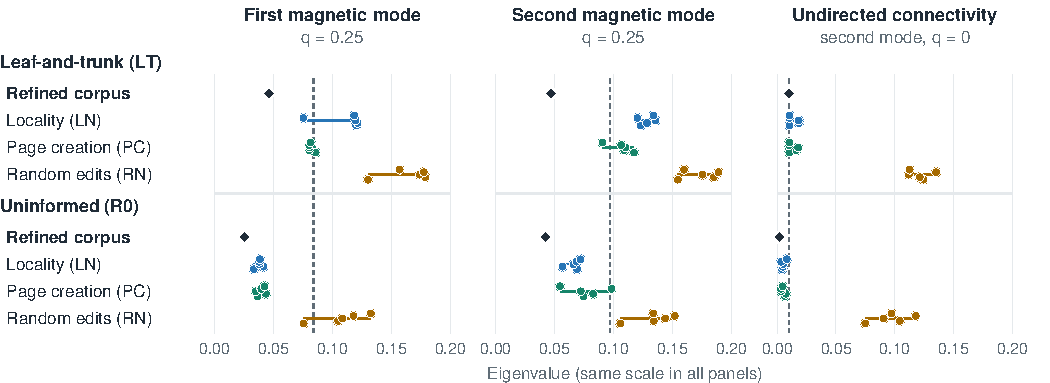
\includegraphics[width=\textwidth]{figures/w02-refinement.pdf}
\caption{Lanes represent refinement styles and their matched controls.
The first magnetic mode is the best-fitting directional pattern; the second
is the next independent pattern. Lower magnetic eigenvalues mean stronger
directional coherence within these patterns, not demonstrated information
flow; lower undirected values mean weaker connectivity. Diamonds show refined
corpora; dots show five controls per row, with segments spanning their range
(not uncertainty). Dashed lines mark original and coincident mapped baselines.
Each graph uses its own LWCC (Table~\ref{tab:refinement-summary}).}
\label{fig:refinement}
\end{figure*}
\begin{table}[t]
\caption{Full-graph pages $N$, links $m$, isolates $I$, mean out-degree $\bar{k}=m/N$ and density $d=m/[N(N-1)]$. LWCC: $n$, $\lambda_1(.25)$ and $F_0$. Area means are LN-standardized LT--R0; rejection threshold $.05$.}
\label{tab:refinement-summary}
\centering
\begin{tabular}{@{}lrrrrrrr@{}}
\toprule
Arm & $n/N$ & $m$ & $I$ & $\bar{k}$ & $d$ (\%) & $\lambda_1$ & $F_0$\\
\midrule
O & 844/1218 & 2494 & 292 & 2.05 & 0.168 & 0.0842 & 0.412\\
LT & 1671/1823 & 5203 & 146 & 2.85 & 0.157 & 0.0462 & 0.314\\
R0 & 1182/1229 & 4502 & 43 & 3.66 & 0.298 & 0.0253 & 0.572\\
\addlinespace
\multicolumn{8}{@{}l@{}}{\textit{Area-paired tests: sample size, mean, $p$}}\\
\multicolumn{8}{@{}l@{}}{Historical (unnormalized): 18, $-0.80$, $0.079$}\\
\multicolumn{8}{@{}l@{}}{Exclude three second-chance areas (unnormalized): 15, $-1.07$, $0.044$}\\
\multicolumn{8}{@{}l@{}}{Normalized (exploratory): 18, $-2.95$, $0.000618$}\\
\bottomrule
\end{tabular}
\end{table}

Both refinements lower LWCC $\lambda_1$, with R0 lowest
(Table~\ref{tab:refinement-summary}); their first two modes fall below their
own LN ranges (Fig.~\ref{fig:refinement}). Ordinary descriptors also separate
edits from nulls. Trophic incoherence falls for LT and rises for R0.

The historical unnormalized test uses area-specific components, LN
standardization and an exact two-sided sign flip, fixed before editing.
It does not reject; excluding second-chance LT areas crosses the threshold
only as a sensitivity result. The smaller normalized $p$-value is exploratory
(Table~\ref{tab:refinement-summary}). Chained areas are not independent realizations.

\begin{table}[t]
\caption{Observed link use: accepted-action shares and trace-level chain. Support is judged at page level. All 1,368 saved traces passed identity/history checks.}
\label{tab:link-use}
\centering
\begin{tabular}{@{}lrr@{}}
\toprule
Measure & LT & R0\\
\midrule
\multicolumn{3}{@{}l@{}}{\textit{Accepted follows}}\\
Added / all accepted & 39/76 & 20/67\\
Mean added-edge menu share & 0.443 & 0.303\\
Added-edge use share & 0.513 & 0.299\\
\addlinespace
\multicolumn{3}{@{}l@{}}{\textit{Trace chain (111 follow-enabled FAQ traces/arm)}}\\
Accepted added-edge follow & 28 & 15\\
First destination-text exposure & 21 & 11\\
Directly supported destination & 7 & 2\\
Cited lines returned by that follow & 7 & 1\\
\bottomrule
\end{tabular}
\end{table}

LT has larger added-edge menu and accepted-follow shares than R0
(Table~\ref{tab:link-use}): greater use accompanies greater availability.
Only a minority of traces reach citation through added-edge use, first exposure
and direct support, more in LT; judged-span overlap is a separate branch.

\begin{figure}[t]
\centering
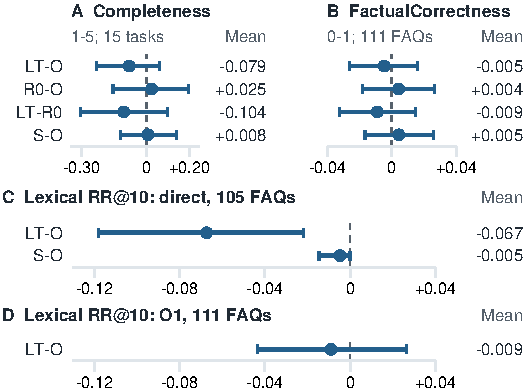
\includegraphics[width=\columnwidth]{figures/w02-answer-intervals.pdf}
\caption{Mean score differences (dots, first minus second) with 95\% intervals
(bars). Positive favors the first arm; including zero means no clear difference,
not equivalence. Metric scales differ; C/D share one. O1 credits moved/derived
content. S--O is replay, not a noise bound.}
\label{fig:answers}
\end{figure}
Primary answer measures show no clear treatment separation
(Fig.~\ref{fig:answers}); the secondary rubric favors R0 over LT but does not
clearly distinguish LT from O. Direct judgments rank LT support lower than O/R0
for lexical and graph-expanded retrieval. The LT--O deficit shrinks under O1,
with an interval spanning zero; the primary replay contrast is much smaller
than the deficit. Embedding retrieval and Recall@5 show no clear separation.
Other O1 gains depend on derived-page credit~\cite{docspectraicsc2027}.

\subsection{A Separate Link-Selection Example}
\label{sec:link-selection-example}
A link-only comparison tests whether magnetic structure changes selection when
semantic assessments tie. Four curated Docker development groups contain
830, 53, 6 and 8 pages. Thirteen candidates wrap existing prose without changing
its words; neither link direction already exists, and endpoints share a baseline
weak component. Each group allows one addition, separately from the LT experiment.

After exposed selector development, Claude Haiku 5.5 and gpt-6.1-sol reviewed
complete source/target pages in isolated requests, blind to prior judgments
and magnetic values. Each scored relationship support, target support and
placement from 0 to 2. Both required every dimension $\geq1$, total $\geq5$,
and no uncertainty or contradiction. Haiku alone sets the admitted semantic
tier; a fixed tie order defines the semantic comparator.

Using the same $W$ and $\theta$ as Section~\ref{sec:magnetic-profile},
page values $e^{i\phi_i}$ of unit magnitude give
\begin{equation}
 E_G(\phi)=\sum_{i<j}2W_{ij}[1-\cos(\phi_i-\phi_j-\theta_{ij})].
 \label{eq:link-phase}
\end{equation}
At $q=.25$, the selector estimates $[F(G+P)-F(G)]/B$ for each candidate $P$,
where $F(G)=\min_\phi E_G(\phi)$ and $B=\sum_{\text{old }i<j}W_{ij}$ stays
fixed for the original group. Unchanged biconnected edge blocks cancel;
changed blocks are solved jointly. Two schedules (seeds 3501/3502), each with
eight L-BFGS-B starts, retain stationary estimates with full-gradient infinity
norm $\leq10^{-7}$. Their extrema measure schedule sensitivity, not error bounds.
A minimum set must have raw envelope spread $\leq10^{-6}$ and every outsider
strictly beyond its upper envelope plus $10^{-6}$; the fixed semantic order
chooses within it. Any unavailable highest-tier option or unresolved overlap
forces whole-tier semantic fallback. Analytic $q=0$ gives the same semantic
choice, without an optimized ordinary-navigation comparator.

All thirteen pass both AI gates. The 53-page language group has eleven options
tied at Haiku 6/6: eight continuous integration and delivery (CI/CD) additions
have raw cost $.194407$, versus $.401924$ for three testing additions.
Here $B=21$. Lower-cost edits create two edge-sharing transitive triangles;
higher-cost edits close two bridges into a triangle. Neither creates a directed cycle.
Restricting the tie order to the eight minima changes .NET
development $\to$ unit tests to C++ development $\to$ CI/CD; cost does not
distinguish C++ from the other seven minima. The Extensions singleton falls
back after nonstationary estimates; Next.js has one option, and the remaining
group has none. Thus only one of four groups is competitive, evaluable and
changed. Actual edits and matched numerical replay were verified.

This is selection behavior on curated, previously inspected examples with
repeated templates, followed by blinded AI support. It supplies neither human
validation nor independent replication. The finite unit-phase cost uses the
magnetic operator's weights and phases; it is not a certified optimum or a
measured decrease in normalized $\lambda_1$, whose eigenvectors allow varying
amplitudes. Retrieval and answer benefit were not tested.


\section{Discussion}
\label{sec:discussion}
The matched reversals establish sensitivity beyond preserved summaries on
observed pairs; cross-corpus correlations cannot isolate this sensitivity
because size and topology also vary. Mostly small, localized and charge-dependent
responses, heterogeneous extraction, selected cycle frames and dependent edits
limit generalization. The measurements distinguish link arrangements without
identifying which serves readers better; that requires evidence about access
and use.

R0's first magnetic eigenvalue is lower than LT's
(Table~\ref{tab:refinement-summary}), despite LT's deliberate organization
around tasks and shared context; this does not establish worse LT information
flow. LT's full-graph density is slightly below the original's after adding pages
and links, whereas R0 is denser. The graphs omit semantic routes and link types;
modes can localize on few pages, and coverage and charge matter. Coupled text,
page and link edits, unequal area acceptance and one corpus per approach limit
interpretation. Metric-guided refinement requires accounting for these influences
and demonstrating useful access; a spectrum alone cannot identify useful links.

Agents used added links without clear primary answer separation; intervals
permit gains and losses. LT's lexical deficit shrinks under moved/derived-content
credit, showing that support attribution matters. Navigation does not establish
answer benefit.

Regression-test prioritization is a possible application, requiring comparison
with simpler change-impact and navigation measures where link traversal
supplies evidence beyond initial retrieval.

\section{Conclusion and Future Work}
This work proposes a reproducible way to characterize directed documentation
structure while making the scope of each comparison explicit. Matched reversals
demonstrate orientation sensitivity beyond preserved summaries in ten corpora.
Docker refinements changed structural profiles and supplied observed link use,
without establishing improved retrieval or answers. Connecting these structural
measurements to better information access remains the next empirical question.

Future work will evaluate more complex tasks in larger documentation
collections, including proprietary corpora, where initial search supplies only
part of the required evidence. These studies will test whether following links
helps complete answers and whether spectral differences identify refinements
that improve this access.

\appendix[Evaluation Checks]
\label{sec:review-appendix}
Author review covered task requirements, support samples and edited content.
Original-corpus support-label agreement was 29/34 positives and 33/33 negatives
(three unsure excluded). Luna's shuffled-reference checks yielded 293/300
scores within $\pm1$ and 11/20 stable rankings (required 80\%); human agreement
was unmeasured. Haiku/RAGAS FactualCorrectness repeat agreement within $.1$ was
78/80 controls and 30/40 development answers (required 90\%). Protocols,
judgments and limitations: DocSpectraICSC2027 v1.1.0~\cite{docspectraicsc2027}.

\section*{Acknowledgments}
OpenAI Codex assisted with drafting the methods exposition in
Section~\ref{sec:design}, rendering mathematics, tables and figures throughout
the paper, and editing manuscript text.
Anthropic Claude Opus assisted with software development.
The authors take responsibility for the content.

\bibliographystyle{IEEEtran}
\bibliography{bibliography/references}
\end{document}
